\documentclass[10pt,twocolumn,letterpaper]{article}
%% Language and font encodings
\usepackage[english]{babel}
\usepackage[utf8x]{inputenc}
\usepackage[T1]{fontenc}
% xcolor is the package between braces and between brackets is the option that we want to use
\usepackage{fancyhdr}
\usepackage{biblatex}
\usepackage{array}
\usepackage[color]{showkeys}
\usepackage{etoolbox}
\usepackage{graphicx,tabularx}
\usepackage{amsfonts} 
%% Sets page size and margins
\usepackage[a4paper,top=3cm,bottom=2cm,left=3cm,right=3cm,marginparwidth=1.75cm]{geometry}
%% Useful packages
\usepackage{amsmath}
\usepackage[colorlinks=true, allcolors=blue]{hyperref}
\fancypagestyle{plain}{%
  \fancyhead{}
  \fancyfoot{}
  \fancyfoot[R]{\thepage}
  \fancyfoot[L]{[INFOMR] Multimedia Retrieval - Utrecht University}
}
\pagestyle{plain}
\title{%
  3D Mesh Retrieval System \\
  \large Multimedia Retrieval \\
    Utrecht University}
    
\author{
  Fabien Da Costa Barros [0720823]\\
  \url{f.n.dacostabarros@uu.students.nl}
  \and
  LastName2, FirstName2\\
  \url{first2.last2@xxxxx.com}
}
\date{\today}
\addbibresource{refs.bib}                                                                     
\begin{document}
\maketitle
\selectlanguage{english}
\section*{Introduction}
The objective of this project is to choose, parametrise and put in practise different procedure and algorithms to build an end-to-end MR System. More precisely the focus will be put on 3D mesh retrieval system. From one mesh we have to retrieve all (at least a decent proportion) of similar mesh. The main challenges will be to analyse different features of a 3D mesh. The main steps of the assignments will be to read and display a 3D mesh; then we have to fix and normalise all the 3D meshes in a database. After that we will extract the feature of the meshes to get the essence of what can define the object is in real life, then compare with other mesh and retrieve similar mesh. At the end we have to improve it so that it can work faster. All of the code can be find on this \href{https://github.com/FDaCostaB/3DMeshRetrievalSystem}{GitHub page}  

\section{Selection and setup the work environment}

We really want to work with Python as both of us as already a good experience and is efficient using it. It is in general easy to set up a new project and install python library and this was one of the main reason of choosing Python for our project. The research of 3D Mesh analysis and visualisation tool as been narrowed to Python libraries. \\ \\
We have discussed the use of PyMesh, PyMeshLab, TriMesh, Open3D, Vedo. To get a nice taste of what each of them can offer we dig in the documentation to compare the differents features. We also complete the step 1 with each of those library to be able to choose after setting up and working (a little) bit with them. \\ \\
	We try to compare the different re-meshing, repairing and extraction features with our current knowledge and thought that PyMeshLab and Open3D seems to be good candidates. Vedo was excluded from the choice at this point as we didn't find enough informations in the documentation even if it looks fancy. Taking into account the short description made on the assignment page of the course's website consolidated our choices as a powerful and reliable library is needed for this project. \\ \\
In this section, four different related packages have been tested and compared. The Comparison of these packages has been done based on several features that might be useful in the future sections of this project. For example, being able to re-mesh objects, scaling them, rotating them, and moving them are the feature that can be useful in the process of normalizing the 3d objects in the database. Also, having some information about the 3d objects, like the number of vertices and faces, is necessary for understanding if these 3d objects are normalized or not. On the other hand, this package must support different formats that are usually used to store 3d objects.
In this case, we narrowed down the packages that work with Python language and well-known between the community. So, we tested and analyzed "Pymesh", "PyMeshLab", "TriMesh", and "Open3D". (See Table \ref{tab:libraries} )\\ \\

	\begin{table*}[t]
    	\hspace*{-0.1\linewidth}\begin{tabular}{|p{0.25\linewidth}|p{0.2\linewidth}|>{\centering}p{0.15\linewidth}|>{\centering}p{0.15\linewidth}|>{\centering}p{0.15\linewidth}|>{\centering\arraybackslash}p{0.15\linewidth}|}
    		\hline
     		Features category & Desired Fetures & PyMesh & PyMeshLab & TriMesh & Open3D \\ \hline
    	    3D format supported & PLY & X & X & X & X \\
    	    ~ & OFF & X & X & X & X \\
    	    ~ & OBJ & X & X & X & X \\
    	    ~ & STL & X & X & X & X \\ \hline
    	    Repairing & Isolated Vertices & X & X & X & To implement \\ 
     		~ & Duplicated Vertices & X & X & X & To implement \\ 
    	    ~ & Duplicated Faces & X & X & X & To implement \\ \hline
    	    Remeshing & Uniform sampling & X & X & X & X \\ \hline
    	    Analysis features & ~ & Simple & Rich & Sufficient & Rich \\ \hline
    	    Visualisation features & Scale & 0 & X & X & X \\ 
   		    ~ & Pan & 0 & X & X & X \\ 
     		~ & Rotate & 0 & X & X & X \\
        	~ & Screenshot & 0 & X & 0 & X \\ 
        	~ & Multiple mesh & 0 & X & 0 & X \\ \hline
        	Language & Source code & 70\% C++ \newline 20\% Python \newline 10\% C  & 80\% C++ \newline 20\%Python & 100\% Python & 80\% C++ \newline 10\% Python \newline 10\% Cuda \\ \hline
        	Number of dependencies & ~ & 7 & 2 & 3 & 0 \\ \hline
        	Interface of preview windows & ~ & None & Advanced & Minimalistic &~ \\ \hline
        	Visualisation interface & Shading methods & None & Flat & Flat & Flat \\ \hline
        	Installation tools & Pip or Anaconda & Docker & Pip & Pip & Pip \\ \hline
    	\end{tabular}
    	 \caption{In-built features for different Python libraries}
  		\label{tab:libraries}
	\end{table*}
	
	We wanted to be able to open "PLY", "OFF", "OBJ", and "STL" formats. "PLY" and "OFF" formats were discussed in the lecture, while "OBJ" and "STL" are really common. All of them were able to open "PLY", "OFF", "OBJ", and "STL" formats, so that was not really discriminating. \\ \\
	We tried to compare the different re-meshing, repairing and extraction features with our current knowledge and thought that PyMeshLab and Open3D seems to be quite good. The complexity was also one of our requirements as from previous experience less complex library offers less options. \\ \\
	After achieving step 1 with four of those libraries (vedo excluded), we try to find a balance between number of dependencies, options proposed for visualizing and analysis. Then we decide to choose "PyMeshLab"\cite{pymeshlab} \\ \\

\section{Step 1}

	For this step, we have done several tries with PyMesh, PyMeshLab, TriMesh and Open3D to get a taste of the different libraries. We get some trouble to set up PyMesh as we have no previous knowledge in Docker. For the other libraries it was really easy to set up and we mainly take advantage of the code snippet of the 'Getting started' page of the corresponding library.  Later on  we will only discuss the PymeshLab project. \\ \\
	Our project have three main dependencies : PyMeshLab, Polyscope and Numpy and run with Python 3.9. At the moment, we have two scripts : main.py and render.py. To have a nice overview and organisation of  the project we will try to split as much as possible the different functionality of the project. 'main.py' just verify the number of arguments and call the function render from 'render.py' with the first arguments passed through. This arguments is the name of the file. We prefer to pass it through the command line so that's it make easy to check tens of mesh and quickly inspect if all is working well. \\ \\
	In 'render.py' there is only one function render() : this function load the mesh, and display the cloud point corresponding to the vertex and the mesh. PyMeshLab have a built-in function '.show\_polyscope' that show a mesh. We find it more interesting to work directly with polyscope to have more control if need to update this later. The result of the mesh visualisation script can be seen at Figure \ref{fig:ant-mesh}. The result of the first step is interesting and satisfy our expectations. The 3D mesh visualisation windows offered a lot of functionality. The look and features offered by PyMeshLab was the most complete library among all of the other libraries tested. 
\begin{figure}
\begin{center}
  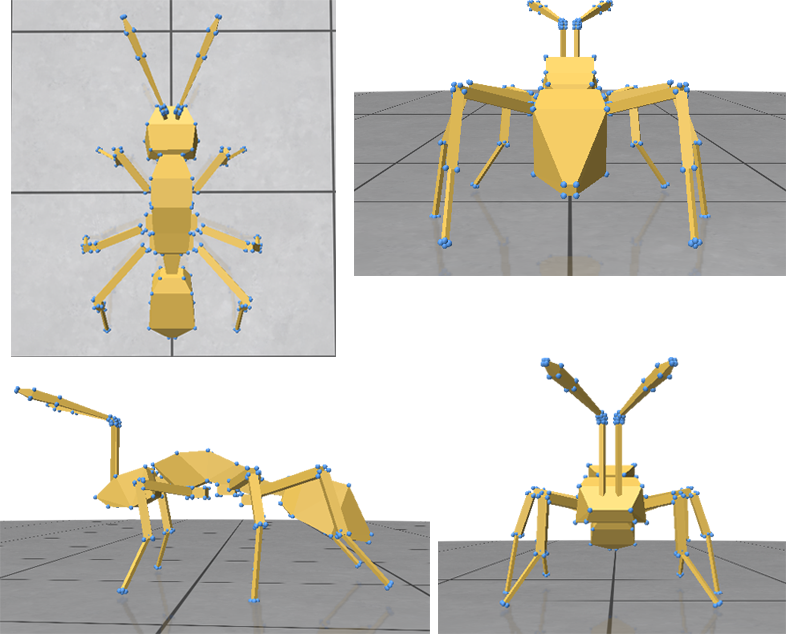
\includegraphics[width=0.5\textwidth]{ant}
  \caption{Visualisation of an ant mesh}
  \label{fig:ant-mesh}
  \end{center}
\end{figure}
%\section*{Acknowledgements}
%Anyone to thank/credit for helping your team along the way? This is the place to do it.
\medskip
\printbibliography
\end{document}